\documentclass[9pt,t]{beamer}
% note that full page width is 12.8 cm and height is 9.6 cm

\mode<presentation>
{
  \usepackage[headline,footline]{beamerthemelectures}

}

% load packages
\usepackage[english]{babel}
\usepackage{graphicx}
\usepackage{multimedia}
%\usepackage[T1]{fontenc}
\usepackage{lmodern}
\usepackage{amsmath,amssymb}
\usepackage{pgf,booktabs,verbatim}
\usepackage{pgfarrows,pgfnodes}
\usepackage[absolute,overlay]{textpos}
\setlength{\TPHorizModule}{\paperwidth}
\setlength{\TPVertModule}{\paperheight}
\usepackage{tikz}

\setbeamertemplate{frametitle}{
\begin{centering}
\insertframetitle
\par
\end{centering}
} 

% create command to add nice looking citation
\newcommand{\reference}[1]{\flushright \vspace{-0.3cm} {\tiny #1}} 


\title{Solutions to Modeling Exercise \#6\\ The global water cycle}

\begin{document}

\section{}

%%%
\frame{
    \frametitle{\vspace{1cm}\huge The global water cycle}
   
}

\frame{
\frametitle{Initial model}
\begin{figure}
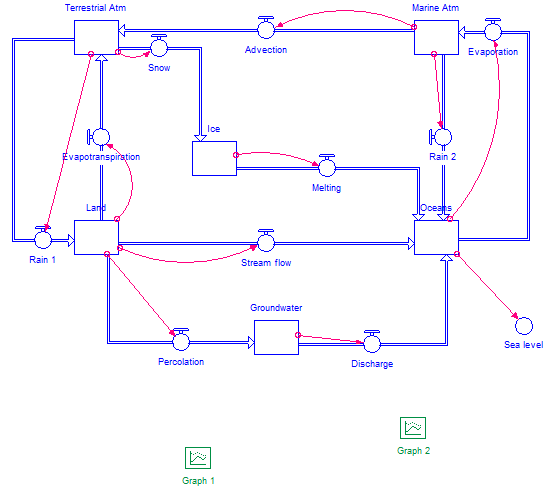
\includegraphics[width=0.8\textwidth]{./initial_model.jpg}
\end{figure}
}

\frame{
\frametitle{1a. Groundwater mining experiment}
\begin{figure}
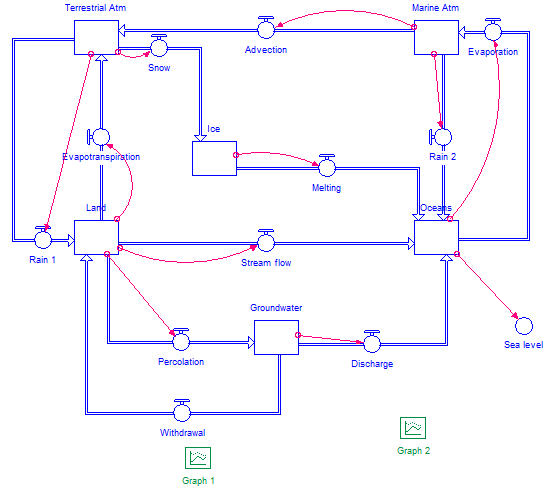
\includegraphics[width=0.8\textwidth]{./gw_mining_model.jpg}
\end{figure}
}

\frame{
\frametitle{1a. Groundwater mining experiment}
\begin{figure}
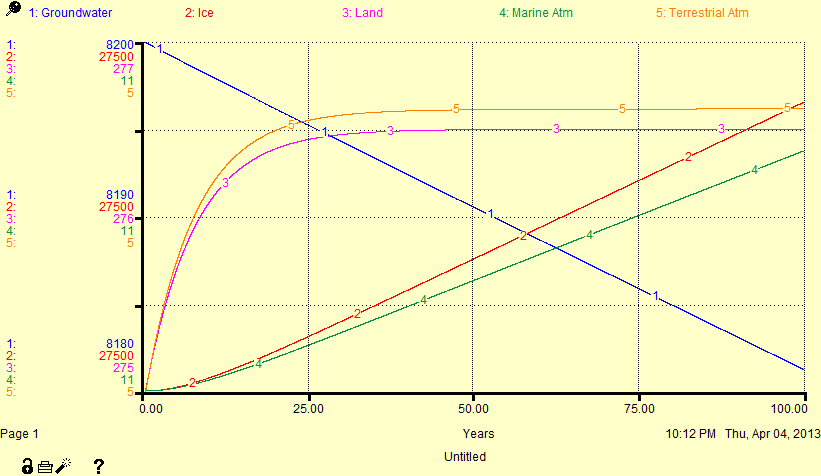
\includegraphics[width=0.9\textwidth]{./p1a-1.jpg}
\end{figure}
\begin{itemize}
\item 
\end{itemize}
}

\frame{
\frametitle{1a. Groundwater mining experiment}
\begin{figure}
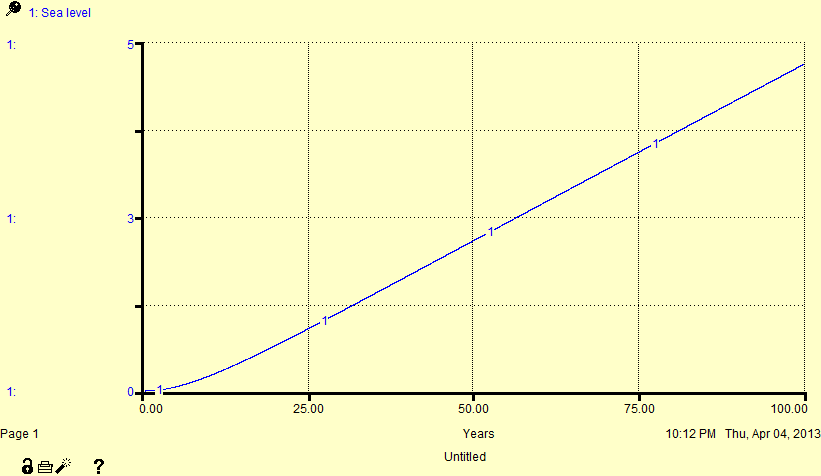
\includegraphics[width=0.9\textwidth]{./p1a-2.jpg}
\end{figure}
\begin{itemize}
\item 
\end{itemize}
}

\frame{
\frametitle{1a. Groundwater mining experiment}
\begin{figure}
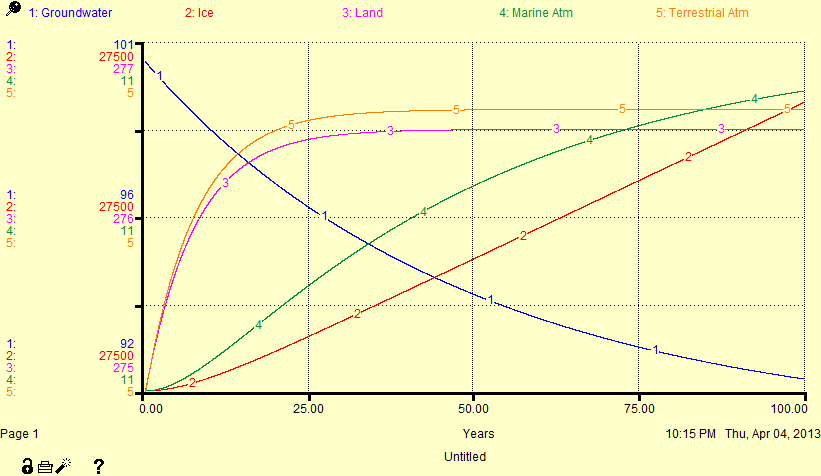
\includegraphics[width=0.9\textwidth]{./p1a-3.jpg}
\end{figure}
\begin{itemize}
\item Smaller groundwater reservoir
\end{itemize}
}

\frame{
\frametitle{1a. Groundwater mining experiment}
\begin{figure}
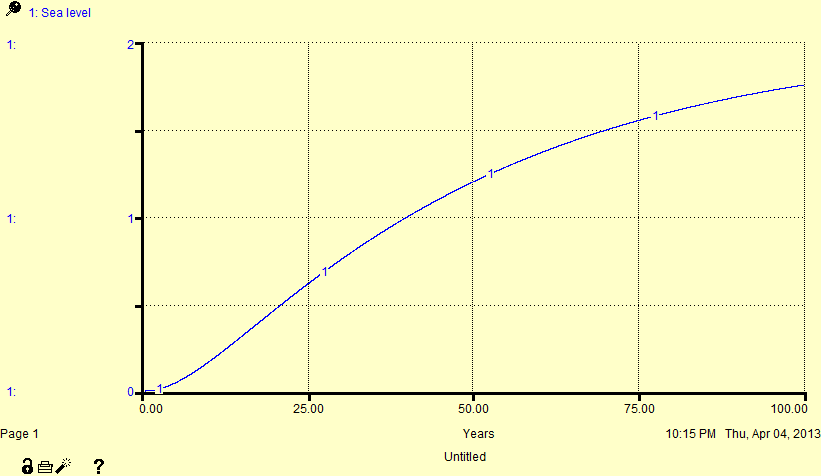
\includegraphics[width=0.9\textwidth]{./p1a-4.jpg}
\end{figure}
\begin{itemize}
\item Smaller groundwater reservoir
\end{itemize}
}



\frame{
\frametitle{1b. Irrigation}
\begin{figure}
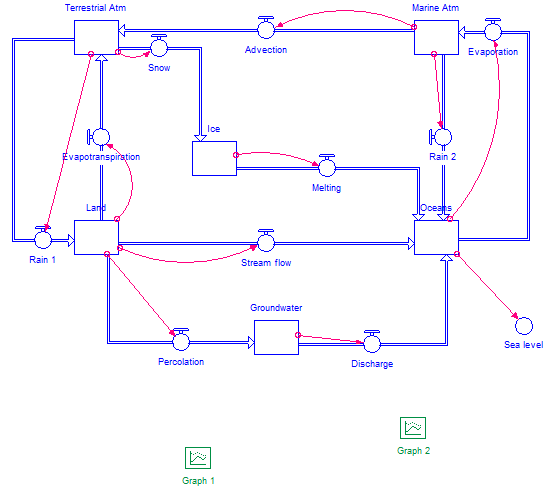
\includegraphics[width=0.8\textwidth]{./initial_model.jpg}
\end{figure}
\begin{itemize}
\item Model irrigation by reducing stream flow
\end{itemize}
}

\frame{
\frametitle{1b. Irrigation}
\begin{figure}
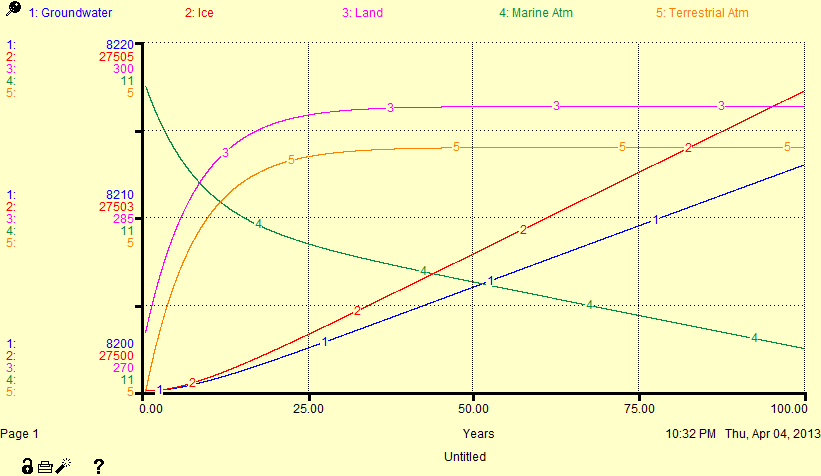
\includegraphics[width=0.9\textwidth]{./p1b-1.jpg}
\end{figure}
\begin{itemize}
\item 
\end{itemize}
}

\frame{
\frametitle{1b. Irrigation}
\begin{figure}
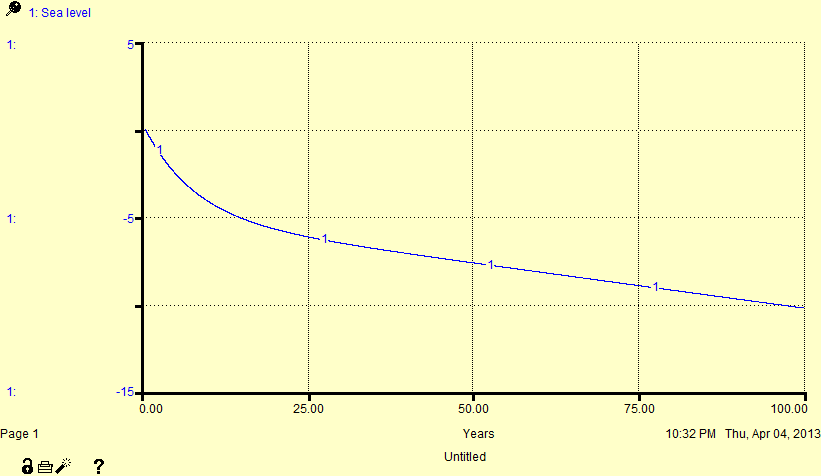
\includegraphics[width=0.9\textwidth]{./p1b-2.jpg}
\end{figure}
\begin{itemize}
\item 
\end{itemize}
}

\frame{
\frametitle{1c. Building dams}
\begin{figure}
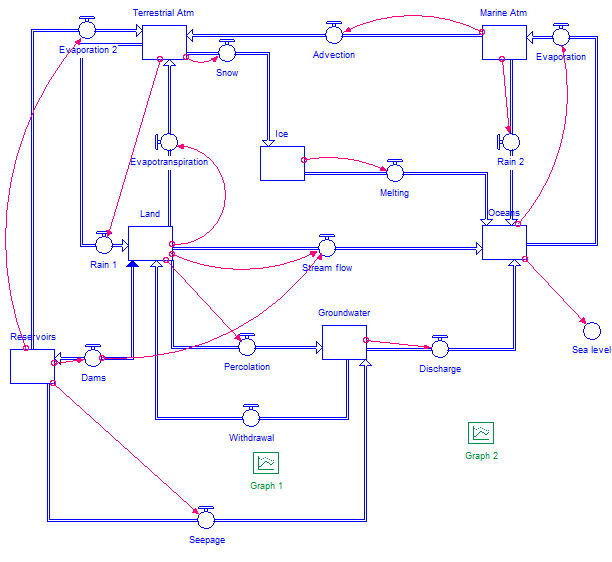
\includegraphics[width=0.8\textwidth]{./dam_model.jpg}
\end{figure}
\begin{itemize}
\item Add reservoir and flows
\end{itemize}
}

\frame{
\frametitle{1c. Building dams}
\begin{figure}
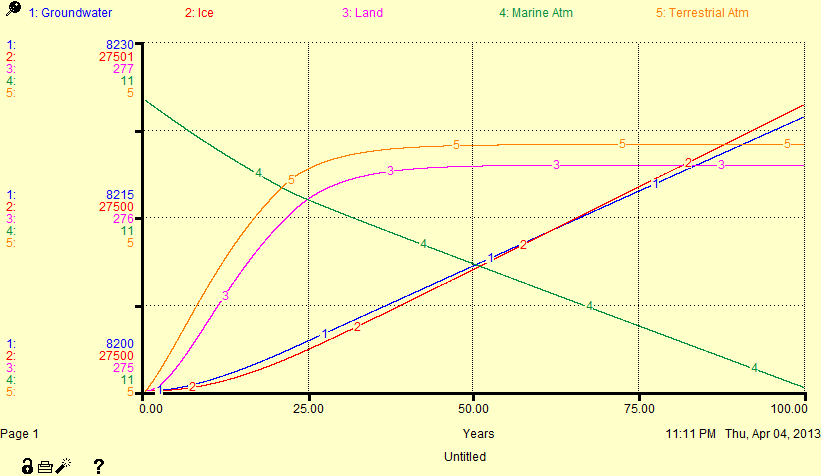
\includegraphics[width=0.9\textwidth]{./p1c-1.jpg}
\end{figure}
\begin{itemize}
\item
\end{itemize}
}

\frame{
\frametitle{1c. Building dams}
\begin{figure}
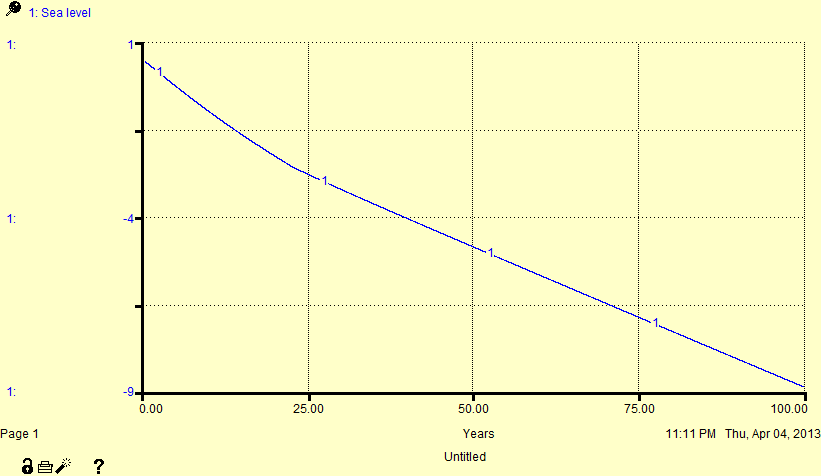
\includegraphics[width=0.9\textwidth]{./p1c-2.jpg}
\end{figure}
\begin{itemize}
\item
\end{itemize}
}

\frame{
\frametitle{1c. Building dams}
\begin{figure}
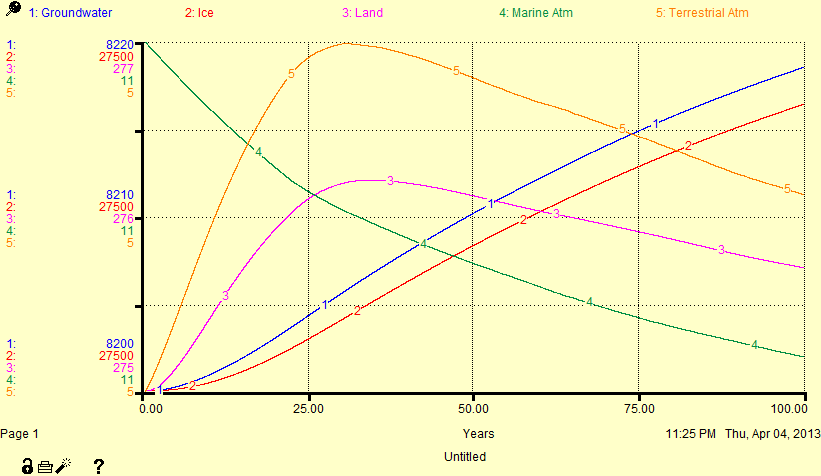
\includegraphics[width=0.9\textwidth]{./p1c-3.jpg}
\end{figure}
\begin{itemize}
\item
\end{itemize}
}

\frame{
\frametitle{1c. Building dams}
\begin{figure}
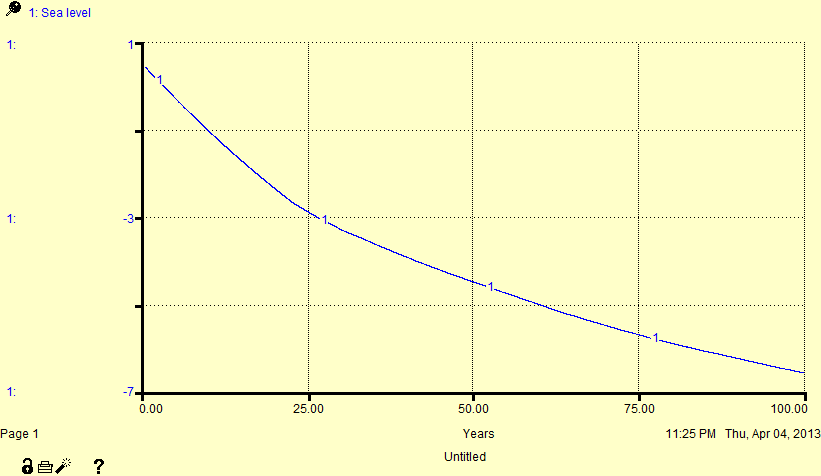
\includegraphics[width=0.9\textwidth]{./p1c-4.jpg}
\end{figure}
\begin{itemize}
\item
\end{itemize}
}

\frame{
\frametitle{2. ``All'' human impacts}
\begin{figure}
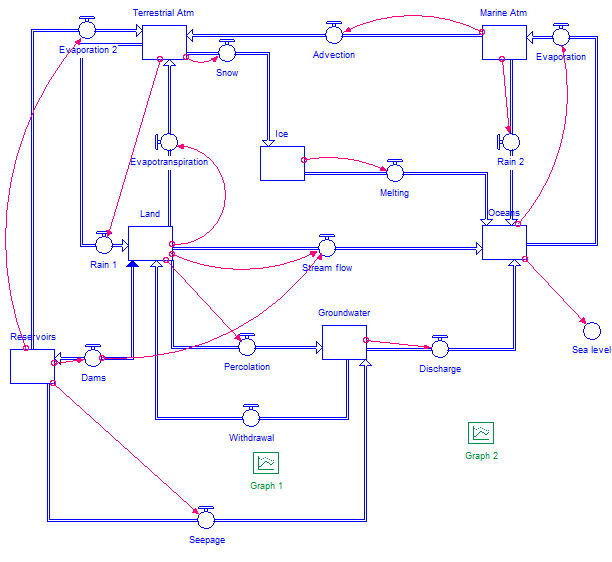
\includegraphics[width=0.8\textwidth]{./all_impacts_model.jpg}
\end{figure}
}

\frame{
\frametitle{2. ``All'' human impacts}
\begin{figure}
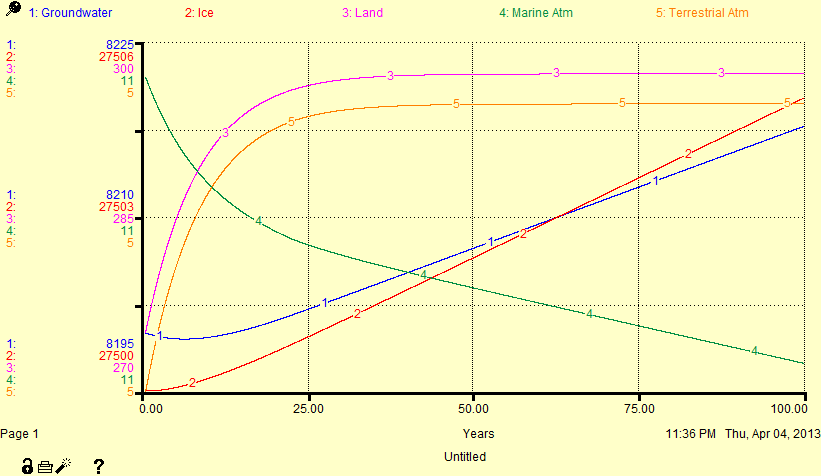
\includegraphics[width=0.9\textwidth]{./p2-1.jpg}
\end{figure}
\begin{itemize}
\item
\end{itemize}
}

\frame{
\frametitle{2. ``All'' human impacts}
\begin{figure}
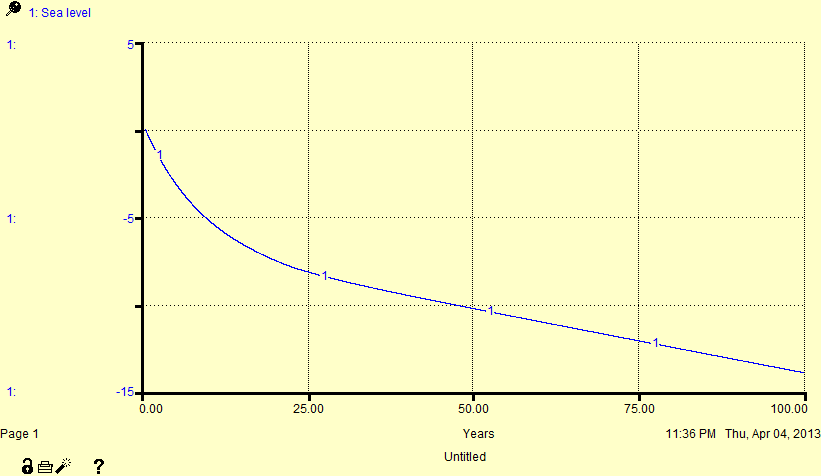
\includegraphics[width=0.9\textwidth]{./p2-2.jpg}
\end{figure}
\begin{itemize}
\item
\end{itemize}
}


\end{document}

\frame{
\frametitle{Key ideas}
\begin{itemize}
\item System parameters can vary unpredictably as a system evolves toward a steady-state
\item The initial conditions matter $\rightarrow$ systems often have multiple steady states; the initial conditions determine which steady state a system will approach
\item Short pertubations can cause a ``permanent'' transition from one state to another
\item Observed a transition out of the (i) cold state for large perturbations in temperature (ii) warm state for moderate perturbations in temperature
\item Also produced transitions from one state to another by modifying the salinity difference
\end{itemize}
}

\end{document}
